\documentclass[aspectratio=169]{beamer}
\usepackage[utf8]{inputenc}
\usepackage[spanish]{babel}
\usepackage{graphicx}
\usetheme{Madrid}
\title{Sombra digital de tráfico en Paute}
\subtitle{Cámara USB, detección vehicular y representación 3D}
\author{David Timbi y equipo}
\institute{Proyecto académico}
\date{\today}
\begin{document}
\begin{frame}\titlepage\end{frame}
\begin{frame}{Problema y objetivo}\begin{itemize}\item Un modelo de tráfico separado del video no refleja el flujo observado en la intersección.\item Integrar cámara local, eventos vehiculares y simulación/visualización.\item Caso: Av. Interoceánica E40 y José Miguel Barzallo, junto al Mercado 26 de Febrero.\end{itemize}\end{frame}
\begin{frame}{Área de estudio}\centering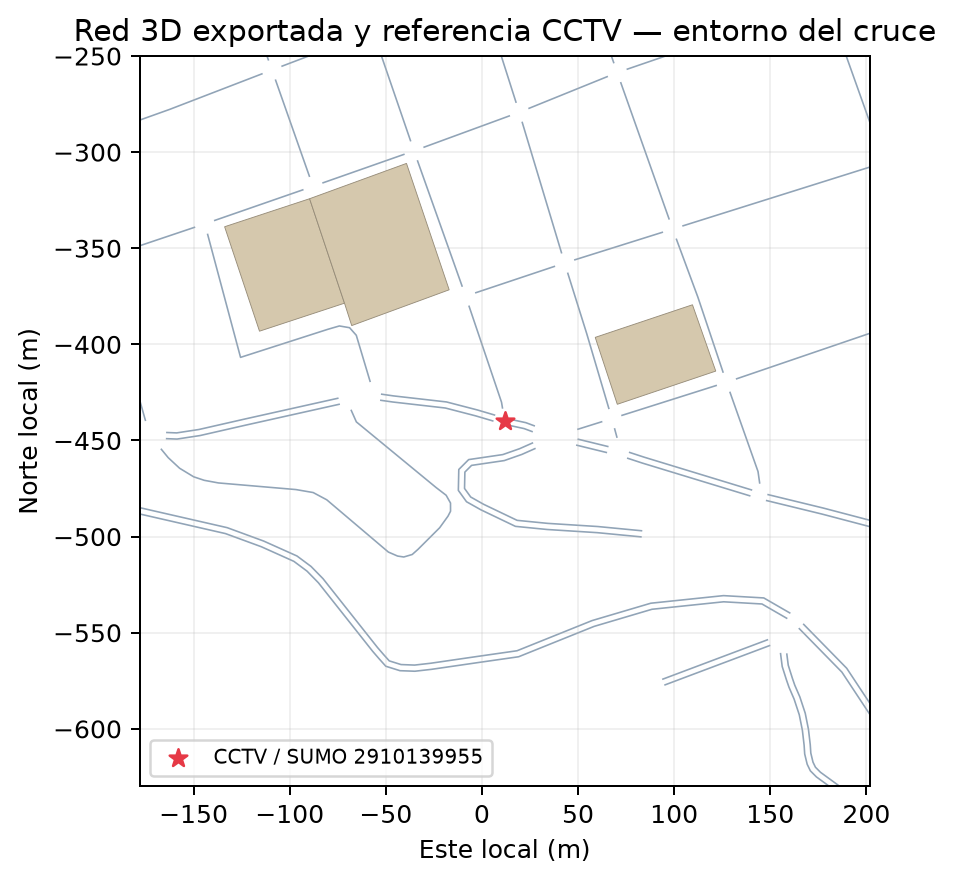
\includegraphics[width=.85\textwidth]{figures/network_junction.png}\\El punto de referencia de cámara es el junction SUMO 2910139955.\end{frame}
\begin{frame}{Arquitectura del prototipo}\centering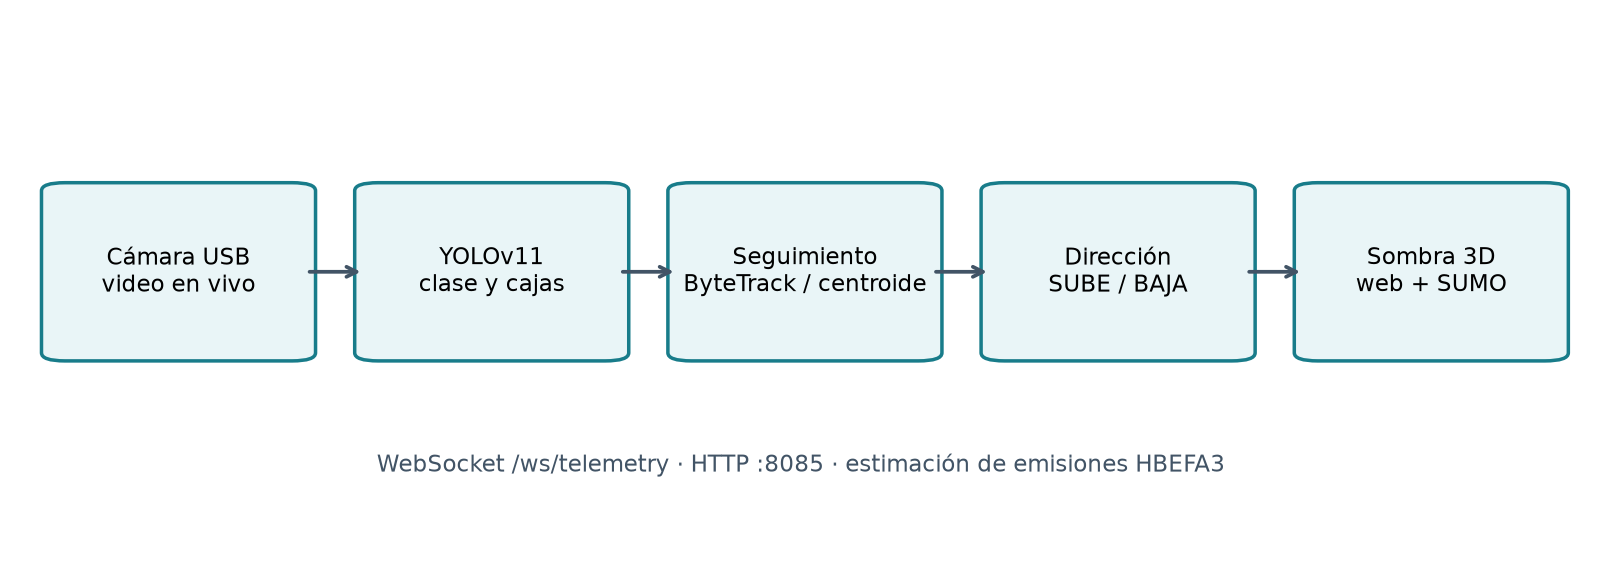
\includegraphics[width=.92\textwidth]{figures/pipeline.png}\end{frame}
\begin{frame}{Qué está implementado}\begin{itemize}\item Red SUMO exportada: 544 aristas, 231 junctions y 29 huellas de edificios.\item Web 3D, HUD, servidor HTTP :8085 y telemetría `/ws/telemetry`.\item YOLOv11 + seguimiento configurado; orientación SUBE/BAJA en eje izquierda/derecha.\item Semilla SUMO 42; paso 0.1 s; conexión TraCI opcional :8813.\end{itemize}\end{frame}
\begin{frame}{Resultados y evidencia}\begin{itemize}\item Verificación del artefacto y configuración reproducible.\item Aún no existe video anotado independiente.\item No afirmar precisión, recall, retraso o error espacial sin matching contra referencia.\item CO$_2$ del HUD es estimación basada en factores, no medición directa.\end{itemize}\end{frame}
\begin{frame}{Evaluación propuesta}\begin{itemize}\item Anotar cruces reales por tiempo, clase, sentido y brazo de entrada/salida.\item Matching uno-a-uno por proximidad temporal/espacial.\item Reportar TP, falsos positivos y omisiones; precision y recall con denominador.\item Medir clase/sentido, demora firmada y error espacial solo con calibración.\end{itemize}\end{frame}
\begin{frame}{Limitaciones y próximos pasos}\begin{itemize}\item Captura autorizada y conjunto anotado; fijar versión/modelo/condiciones.\item Validar motos, buses, oclusión y sentido BAJA.\item Comparar con baseline SUMO calibrado y revisar rutas conectadas.\item Agregar replay offline y resultados reproducibles con tag Git.\end{itemize}\end{frame}
\begin{frame}{Cierre / preguntas}\centering\Large Prototipo funcional; validación de campo pendiente.\\[1em]10 min exposición + 5 min preguntas\end{frame}
\end{document}
